\documentclass[10pt]{article}

\usepackage[utf8]{inputenc}
\usepackage[portuges]{babel}
\usepackage{a4wide}
\usepackage{graphicx}
\usepackage[export]{adjustbox}
\usepackage[labelformat=empty]{caption}
\graphicspath{ {img/} }

\begin{document}

\title{Projeto de Laboratórios de Informática 3\\Grupo 34}
\author{Alexandre de Freitas Ferreira Pacheco A80760\and Diogo José Cruz Sobral A82523\and José Pedro Milhazes Carvalho Pinto A80741}


\date{\today}


\maketitle

\begin{figure}[h]
	\minipage{0.32\textwidth}\centering
		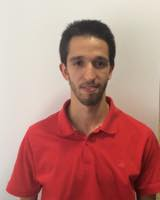
\includegraphics[scale=0.5]{A80760.png}
		\caption{A80760}
		\label{fig1:A80760}
	\endminipage\hfill
	\minipage{0.32\textwidth}\centering
		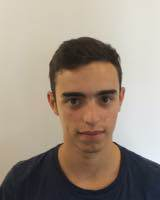
\includegraphics[scale=0.5]{A82523.jpg}
		\caption{A82523}
		\label{fig2:A82523}
	\endminipage\hfill
	\minipage{0.32\textwidth}\centering
		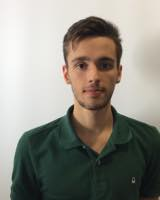
\includegraphics[scale=0.5]{A80741.jpeg}
		\caption{A80741}
		\label{fig3:A80741}
	\endminipage
\end{figure}


\begin{abstract}
		Nesta unidade curricular foi-nos proposta a implementação de um sistema
	de resposta a \textit{queries} sobre um \textit{dump} da  base dados do site
	 \emph{Stack Overflow}.
	
		A primeira fase deste projeto consistiu no desafio de implementar este
	sistema na linguagem \emph{C}. Era permitido (e recomendado) o recurso a
	bibliotecas como, por exemplo \textit{libxml2} ou a \textit{glib}.
	Apesar da intenção de tornar rápida a execução das funcionalidades do programa
	a ser desenvolvido, alguns dos focos prioritários deste projeto foram
	a modularidade e o encapsulamento das estruturas de dados por nós utilizadas.
	
		Note-se que estas preocupações vão de encontro à aprendizagem realizada 
	neste semestre no âmbito da programação orientada aos objetos, bem como ao
	objetivo da segunda fase do projeto, que consiste na implementação do mesmo
	sistema na linguagem \emph{Java}.

		Ao longo do desenvolvimento deste projeto, consideramos que os maiores 
	desafios foram implementar as estruturas onde organizar a informação, e, sobretudo, 
	encontrar o \textit{sweet spot} do compromisso segurança vs. rapidez.   
\end{abstract}

\pagebreak

\section{Ferramentas Utilizadas} 

		Como referido, este projeto, desenvolvido em C, podia ser auxiliado por 
	diversas ferramentas. 
	
		Em relação ao parsing dos ficheiros \emph{.xml} sob
	a forma dos quais era disponibilizado o \textit{dump}, optámos por utilizar a biblioteca
	\textit{libxml2}, por uma questão de comodidade.
	
		Para construir as nossas estruturas de dados, decidimos criar os nossos 
	próprios módulos em vez de utilizar totalmente \textit{glib}, a fim de obter ferramentas
	que, embora não tão robustas quanto as desta biblioteca, apresentam todas as
	características necessárias neste projeto e uma simplicidade que se traduz numa
	vantagem no que toca à rapidez em algumas operações.
	
		Ainda assim, recorremos ao \textit{glib} para implementar uma pequena parte
	da nossa estrutura de dados e para nos ajudar a responder algumas \textit{queries}.
	
	
\section{Tipos e Estruturas de Dados}		

		De modo a conseguir responder às \textit{queries} propostas de forma eficiente, é natural
	que o mais importante é a forma como organizamos o grande volume de informação 
	presente nos \textit{dumps} disponibilizados.
		
		Primeiro, analisámos a informação contida em cada um dos ficheiros \textit{xml}
	disponibilizados por comunidade (e.g. \textit{android}, \textit{ubuntu}...) e o 
	que era pedido nas \textit{queries}, a fim de perceber quais os dados que seriam recorrentemente
	necessários.
	
\subsection{Tipos de Dados: \textit{Users} e \textit{Posts}}
	
		As entidades elementares na forma de descrever cada comunidade, à volta das quais
	gira a grande maioria da informação, são os \textit{users} e os \textit{posts}.
		Naturalmente, para cada um destes objetos criámos um tipo de dados próprio, 
	\texttt{MYUSER} e \texttt{MYPOST}.
	
\begin{figure}[h]
	\begin{minipage}{.5\textwidth}
		\includegraphics[scale=0.5]{mypost.png}\centering
		\caption{\texttt{typedef struct mypost * MYPOST;}}
		\label{fig4:mypost}
	\end{minipage}
	\begin{minipage}{.5\textwidth}
		\includegraphics[scale=0.5]{myuser.png}\centering
		\caption{\texttt{typedef struct myuser * MYUSER;}}
		\label{fig5:myuser}
		
		\includegraphics[scale=0.5]{stackpost.png}\centering
		\caption{\texttt{typedef struct stackpost * STACKPOST;}}
		\label{fig6:stackpost}
	\end{minipage}
\end{figure}	

\pagebreak	
\subsection{Organização das Estruturas Elementares}
		
		Criados os tipos de dados dos \textit{users} e \textit{posts}, procedemos 
	à implementação da organização dos mesmos, fator determinante na viabilidade e 
	qualidade deste projeto.
	
		Decidimos organizar os \textit{users}, bem como os \textit{posts} em árvores
	binárias de procura balanceadas. Optámos ainda por utilizar duas árvores para
	organizar os \textit{posts}, uma em que as chaves de ordenação são o \textit{Id} do 
	\textit{post},	e outra em que as chaves são as datas de criação (e em que em cada
	nodo da árvore há um \textit{array} de \textit{posts} criados no mesmo dia).
	
		É importante mencionar que os nodos das árvores não contêm a informação que
	nelas se organiza, propriamente dita, mas sim um apontador para as estruturas
	elementares que a armazenam, e permitindo assim a partilha dessas "cápsulas de informação"
	entre diversas estruturas criadas para as organizar e percorrer de forma diferente.
	
\subsection{Outras Estruturas Auxiliares}
		
		Para além da organização essencial referida, decicidmos implementar, ainda, 
	estruturas auxiliares, que são úteis sobretudo quando a resposta a determinadas
	\textit{queries} envolve calcular um conjunto de perguntas mais respondidas ou 
	um conjunto de	utilizadores com maior reputação.
	
		Duas destas estruturas são \textit{heaps}. Uma armazena as reputações de todos os
	users, outra armazena o número de posts de cada user. Estas \textit{heaps} são
	criadas e preenchidas logo após a construção das árvores referidas anteriormente.
	
		Outras duas estruturas são \textit{stacks} que estão de certa forma relacionadas
	com as \textit{heaps}. Estas são apenas construídas quando é necessário calcular
	um conjunto de N utilizadores com maior reputação, ou com maior número de posts.
	Após serem construídas, ficam guardadas e podem crescer se for necessário obter
	novamente um conjunto semelhante mas com um número maior que N.
		Assim, há cálculos que após serem efetuados uma vez, deixam de ter de ser efetuados,
	na mesma \textit{query} e mesmo entre \textit{queries} diferentes.

		Utilizámos ainda uma tabela de \textit{hash} da biblioteca \textit{glib},
	que armazena as \textit{tags} como chaves e os \texttt{Ids} das \texttt{tags}
	como valor correspondente.
	
\begin{figure}[h]
	\begin{minipage}{.5\textwidth}\centering
		\includegraphics[scale=0.5]{comm.png}
		\caption{\texttt{typedef struct TCD\_community * TAD\_community;}}
		\label{fig7:community}
	\end{minipage}
	\begin{minipage}{.5\textwidth}\centering
		\includegraphics[scale=0.5]{heap.png}
		\caption{\texttt{typedef struct heap * HEAP;}}
		\label{fig8:heap}
	\end{minipage}
	
\end{figure}	
	
	A nossa \texttt{HEAP} é uma \textit{max-heap}, no entanto, construímo-la
de modo a que, nos casos em que dois elementos da \textit{heap} têm chaves iguais,
estes estão ordenados pelo seu valor \texttt{data} de forma crescente. Por
exemplo, se estamos a organizar \texttt{Ids} de \textit{tags} pelo número de
ocorrências (como na \textit{query} 11), e as \textit{tags} 10 e 20 têm as mesmas 
ocorrências, então a 10 fica acima da 20.
	
\pagebreak

\section{Modularização e Abstração de Dados}
		Como temos aprendido ao longo dos últimos tempos, são boas práticas as de 
	manter um código modular e abstraído do tipo de dados com que	trabalhamos.
	
	\subsection*{Encapsulamento}
	
		Seguindo este pensamento, separámos as partes funcionais do nosso programa
	em diferentes módulos e deixámos o mínimo de funções visíveis para o exterior. As
	funções que podem ser chamadas de fora do módulo (por exemplo os \textit{"gets"})
	devolvem sempre uma cópia da informação contida na nossa estrutura, de modo a não
	comprometer o encapsulamento dos nossos tipos de dados e, por conseguinte, a integridade
	da estrutura da montada.
	
	
\begin{figure}[h]
\centering
		\begin{minipage}{.5\textwidth}\centering
		\includegraphics[scale=0.5]{getname.png}
		\caption{Exemplo de método \textit{get} a clonar informação.}
		\label{fig9:getname}
	\end{minipage}
\end{figure}
	
		Um sistema de proteção que implementámos consistiu em ter uma variável dentro de 
	cada tipo (por exemplo um \texttt{MYPOST} ou \texttt{MYUSER}) que especifica se a
	\textit{struct} em questão é ou não uma cópia. Se for uma cópia pode ser libertada
	normalmente, mas se for a instância "original" (a construída no \texttt{load}), apenas 
	pode ser libertada por funções que não são visíveis para fora (e que apenas são chamadas na
	função \texttt{clean}.
	
	
	\subsection*{}
		Para além disso, tivemos também o cuidado de escrever código "neutro" em 
	relação a tipo de dados. A nossa implementação de árvores binárias de procura 
	balanceadas, por exemplo, trabalha com chaves e valores do tipo \texttt{void *}
	de modo a podermos a qualquer altura mudar a organização da árvore, ou criar uma
	nova, apenas escrevendo uma função de comparação (para as \textit{keys}) e funções
	para libertar os dados usados.

\begin{figure}[h]
\centering
		\begin{minipage}{.5\textwidth}\centering
		\includegraphics[scale=0.5]{trees.png}
		\caption{\texttt{typedef struct tree * TREE;}}
		\label{fig10:tree}
	\end{minipage}
\end{figure}
\pagebreak

\section{\textit{Queries}}
		Nesta secção passamos a explicar a abordagem que tomámos em relação
	a cada uma das \textit{queries}. 
	\subsection*{\textit{Query} 1 - Título e autor da pergunta}
		O procedimento que tomamos é bastante simples. 
		\begin{enumerate}
		\item Procuramos o post com o \texttt{Id} fornecido e verificamos se se trata
		 de uma pergunta. 
		\begin{enumerate}
		\item Se for uma pergunta, devolvemos o seu título e o \texttt{DisplayName} do autor 
	(procurado o \texttt{OwnerUserId} na árvore de users).
	
		\item Se for uma resposta, repetimos o ponto \textbf{1} com o \texttt{ParentId}
		do post, que será o \texttt{Id} da pergunta correspondente.
		\end{enumerate}
		\end{enumerate}
	\subsection*{\textit{Query} 2 - Top N \textit{users} com mais posts}
			Esta query toma partido da heap de utilizadores ordenados pelo seu número de posts
		que construímos na \texttt{load} e da \textit{stack} de \texttt{Ids} de users
		organizados pelo número de posts que preenchemos à medida que as \textit{queries}
		chamadas necessitam. 
		\begin{enumerate}
			\item Inicializa-se a \texttt{LONG\_list} com N elementos e verifica-se se a
			\textit{stack} de \texttt{Ids} de utilizadores organizada por número de posts 
			tem N ou mais elemntos.
			\begin{enumerate}
				\item Se tiver N ou mais elementos, então, a essa \textit{stack} é percorrida
				e preenche-se a lista resultado.
				\item Se tiver menos de N elementos, então percorre-se os elementos que esta
				já tem preenchendo-se a lista resultado, e depois, até haver N elementos na
				\textit{stack}, faz-se \textit{pop} à \textit{heap} e inserem-se os elementos
				que vão sendo colocados na \textit{stack} também na lista resultado.
			\end{enumerate}
		\end{enumerate}			
	\subsection*{\textit{Query} 3 - Número de perguntas e respostas ao longo de um período}
			Como já referido, a árvore que organiza os \textit{posts} por data, em cada nodo,
		tem um array de posts. Para além do array propriamente dito, com apontadores do tipo
		\texttt{MYPOST}, há dois contadores: um para o número de respostas, e outro para o
		número de perguntas nesse array (calculados no \texttt{load}). Ora, é desta organização
		que esta \textit{query} toma partido.
		\begin{enumerate}
			\item Percorre-se os nodos da árvore de posts dentro do período especificado.
			
				Em cada nodo da árvore, soma-se os respetivos contadores à variável cujo 
			endereço é passado como argumento pela função de travessia.
		\end{enumerate}
	\subsection*{\textit{Query} 4 - Perguntas com determinada \textit{tag} feitas num período}
		\begin{enumerate}
			\item Percorre-se todos os nodos da árvore de posts dentro do período especificado.

				Percorre-se o \textit{array} de posts em cada nodo, e em cada post verifica-se
			se este é uma pergunta e contém a tag especificada. Se for esse o caso, adiciona-se
			o \texttt{Id} a um \textit{array} resultado (de onde posterioremente se passarão
			os valores para \texttt{LONG\_list})

		\end{enumerate}
			
	\subsection*{\textit{Query} 5 - Informação de um \textit{user} e os seus últimos \textit{posts}}
			Esta \textit{query} consiste em simplesmente procurar um utilizador na nossa estrutura
		e devolver a sua informação.			
			O tipo de dados \texttt{MYUSER} contém, como já foi visto, um \textit{array} com
		os \texttt{Ids} dos seus posts,o que facilita imenso esta resposta.
	\subsection*{\textit{Query} 6 - N respostas mais votadas ao longo de um período}
			A diferença entre os \textit{upvotes} e \textit{downvotes} de uma resposta
		equivale ao seu parâmetro \texttt{Score}, pelo que este já se encontra calculado
		a partir do momento em que o carregámos do ficheiro \textit{xml}.
			\begin{enumerate}
				\item São visitados todos os nodos da árvore de \textit{posts} dentro
					do período especificado, percorrendo o \textit{array} de \textit{posts}
					em cada nodo e inserindo numa \texttt{HEAP} (\textit{max-heap}) o par de
					informação \{\texttt{Id}, \texttt{Score}\}.
				\item Dá-se \textit{pop} a N elementos da heap e preenche-se a lista 
					resultado com os \texttt{Ids} das respostas a ser retiradas da \textit{heap}.
			\end{enumerate}
	\subsection*{\textit{Query} 7 - N perguntas com mais respostas ao longo de um período}
			Dado que as respostas às perguntas a devolver têm de ter sido feitas ao longo
		do período especificado, esta \textit{query} não se resume a consultar o número
		de respostas em cada pergunta no período de tempo, mas a calcular o número de 
		respostas feitas ao longo desse período para cada pergunta.
			\begin{enumerate}
				\item Percorre-se todos os \textit{posts} criados no período de tempo
					dado.
					\begin{enumerate}
						\item Percorre-se a lista de filhos desse \textit{post} (que só
							existe se este for uma pergunta) e conta-se quantos foram
							criados no período de tempo especificado.
						\item Insere-se numa \texttt{HEAP} (\textit{max-heap}) o par de  
							informação \{\texttt{Id}, número de respostas\}.
					\end{enumerate}
				\item Faz-se \textit{pop} a N elementos da \textit{heap}, guardando 
					na lista resultado os \texttt{Ids} das perguntas nas condições
					especificadas.
			\end{enumerate}
	\subsection*{\textit{Query} 8 - N perguntas mais recentes com determinada \textit{tag}}
			A query 8 não exige que todos os \textit{posts} sejam consultados,
		uma vez que estes se encontram organizados por tempo, e assim, podemos obter tudo o que 				precisamos visitando o número	mínimo de posts.
		
			O critério que utilizámos para determinar se a palavra ocorre ou não em cada
		título (para além de obviamente essa sequencia de caracteres aparecer na \textit{string}
		do título) foi a existência de espaços, pontuação, \textit{newline} ou \texttt{EOF}
		nas extremidades da \textit{substring} com a palavra. Para nos facilitar este trabalho
		utilizámos as funções de biblioteca \texttt{ispunct()} e \texttt{isspace()}.
			\begin{enumerate}
				\item Efetua-se uma travessia semelhante à \textit{inorder} na ordem
					"posts recentes - posts antigos". Que termina quando todos os
					nodos da árvore tiverem sido percorridos ou quando obtivermos N
					\textit{posts} nas condições pretendidas.
					\begin{enumerate}
						\item	Em cada nodo, percorre-se o array de \texttt{MYPOST}, e em cada 
						\textit{post} verifica-se se este contém a \textit{tag} especificada.
						Sendo esse o caso, adiciona-se o \texttt{Id} do \textit{post} a um
						\textit{array} (que posteriormente é passado para a \texttt{LONG\_list} 
						resultado).
					\end{enumerate}
			\end{enumerate}
	\subsection*{\textit{Query} 9 - N perguntas mais recentes em que dois \textit{users} participaram}
			Esta é outra query em que se tira bastante partido do facto de termos, no \texttt{load},
		carregado para o tipo \texttt{MYUSER} um array \texttt{STACKPOST} com os posts de cada
		\textit{user}.
			\begin{enumerate}
				\item São procurados os dois \textit{users} a partir dos \texttt{Ids} especificados e verifica-se qual dos dois tem menos posts.
				\item São percorridos os \textit{posts} desse user e são inseridos numa tabela
de \textit{hash} os \texttt{Ids} das perguntas relativas a cada post (ou seja, o próprio
\texttt{Id} se o \textit{post} for uma pergunta, ou o \texttt{ParentId} se o mesmo for uma
resposta).
				\item É repetido o processo para o outro utilizador, mas em vez de se inserir
na tabela \textit{hash} os \texttt{Ids}, verifica-se se estes estão já inseridos na tabela.
Aqueles que já estiverem são constituintes do reultado, sendo armazenados num \textit{array}
\texttt{STACKPOST}.
				\item Os elementos deste \textit{array} são ordenados segundo um algoritmo
\textit{quicksort} (segunda a sua \texttt{CreationDate}, e os N mais recentes são passados
para a \texttt{LONG\_list} resultado.
			\end{enumerate}
	\subsection*{\textit{Query} 10 - Melhor resposta}
			Esta \textit{query} é relativamente simples, devido ao facto de no \texttt{load} 
			armazenarmos um \textit{array} \texttt{STACKPOST} que guarda as respostas a cada 
			pergunta.
			\begin{enumerate}
				\item É procurada a pergunta na árvore ordenada por \texttt{Ids}.
				\item É percorrido o \texttt{STACKPOST} das respostas à pergunta e para cada
					um deles é calculada a pontuação (segundo a fórmula especificada no enunciado)
					e registado a melhor pontuação bem como a respetiva resposta, cujo \texttt{Id}
					é depois retornado. 
			\end{enumerate}
	\subsection*{\textit{Query} 11 - N \textit{tags} mais usadas ao longo de um período pelos N \textit{users} com maior reputação}
			Esta \textit{query} faz uso de grande parte das estruturas que temos montadas, bem
		como de estruturas criadas ao longo da sua execução.
		
			Nesta query, é criada uma tabela de \textit{hash} com as ocorrências de cada
		\textit{tag}. É ainda criada uma \texttt{HEAP} (\textit{max-heap}) onde depois são inseridos
		os \texttt{Ids} das \textit{tags} e as suas ocorrências como chave, de modo a ficarem 
		ordenados.
			É ainda importante mencionar que, na nossa interpretação do que foi pedido,
		utilizámos os N utilizadores com maior reputação de sempre (mesmo que não tenham
		postado nesse período de tempo). No resultado da query, \texttt{Ids} de tags com
		o mesmo número de ocorrências estão em ordem crescente.		
		
			\begin{enumerate}
				\item É obtido um array com os \texttt{Ids} dos N \textit{users} com
					maior reputação (procedendo da mesma forma que na \textit{query} 2, mas em
					relação à reputação e não ao número de posts).
				\item O array obtido é percorrido, procurando cada \texttt{Id} na árvore dos
					\textit{users} e obtendo  o \texttt{STACKPOST} com os \textit{posts}
					criados por cada um desses utilizadores.
					\begin{enumerate}
						\item Se o \textit{post} for uma pergunta e tiver sido criado dentro
							do intervalo de tempo especificado;
						\item Percorre-se cada \textit{tag} desse \textit{post} e, consultando 
						 a tabela de \textit{hash} pré-calculada, obtém-se o \texttt{Id} da mesma.
						\item Se este \texttt{Id} já constar na outra tabela de \textit{hash} que
							faz corresponder cada \texttt{Id} ao seu número de ocorrências, é 
							incrementado esse número. Caso contrário, esse \texttt{Id} é inserido.
					\end{enumerate}
				\item Preenchida a tabela \textit{hash} que a cada \texttt{Id} faz corresponder
				o seu número de ocorrrências, percorre-se todas as entradas da mesma e insere-se
				o par \{número de ocorrências, \texttt{Id}\} numa \textit{max-heap}, ficando assim
				os \texttt{Ids} ordenados.
				\item É feito \textit{pop} de N elementos da \texttt{HEAP}, e preenche-se a
				\texttt{LONG\_list} resultado com os \texttt{Ids} desses elementos.
			\end{enumerate}
\pagebreak

\section{Estratégias para melhorar a Eficiência}
		Tendo em conta o grande volume de dados que nos propusemoss a processar neste projeto,
	surge a necessidade de adotarmos estratégias que melhorem a eficiência das operações que
	levamos a cabo.
	
		Uma prática que procurámos ter foi a utilização de arrays sempre que possível. Um bom 
	exemplo da nossa "aproximação" aos \textit{arrays} é a nossa implementação de \textit{max-heaps} 
	que utilizámos frequentemente para armazenar e retirar ordenadamente elementos para respostas 
	a \textit{queries}.
	
		Outra forma de tornar o nosso programa mais eficiente foi, durante o \texttt{load},
	construir estruturas auxiliares que, embora armazenassem informação que pudesse ser obtida
	a partir das árvores de \textit{posts} e \textit{users}, e levassem a um ligeiramente maior
	gasto de memória, eram úteis a muitas \textit{queries} e poupavam imensos cálculos e travessias.
	
		Aproveitar a organização das estruturas de dados para os percorrer de diferentes maneiras,
	consoante a necessidade, foi também uma opção que tornou a nossa resposta a certas 
	\textit{queries} mais eficiente, como por exemplo, a existência de várias travessias nas 
	árvores binárias balanceadas de procura, ou, como já referido, a utilização da \textit{max-heap}
	para criar mapas ordenados.

\section{Conclusão}
	Atingidos os objetivos deste projeto, retivemos alguns prontos principais.
	
	Primeiro, a necessidade de abdicar de performance para ter um código seguro,
protegido não só do utilizador comum mas principalmente de terceiros que pretendam 
aceder e possivelmente modificar uma estrutura de dados.

	Outra observação foi a importância da organização das estruturas de dados, a 
influência destas nos algoritmos a aplicar, e como diferentes combinações
destes dois conceitos tiveram um impacto palpável nos tempos de execução das
funcionalidades do programa.	
	
	Por fim, não pudemos deixar de notar no facto de que C, por ser uma linguagem 
de baixo nível de abstração, carece de funcionalidades que outras linguagens
(\textit{e.g.} \textit{Java}, \textit{Python}...) apresentam e facilitam o trabalho do
programador (não tendo este de "reinventar a roda"). Assim, esperamos que a segunda fase deste trabalho (implementação
em \textit{Java}) seja mais simples de realizar, ainda que com uma penalização na performance.

\end{document}\grid
\grid\grid
\grid
